\documentclass{article}
\usepackage[margin=2cm, a4paper]{geometry}
\usepackage{blindtext}
\usepackage{ctex}
\usepackage{longtable}
\usepackage{tabularx}
\usepackage{amsmath}
\usepackage{tikz}
\usepackage{multicol}
\usepackage{titling}
\usepackage{graphicx}
\usepackage{listings}
\usepackage{float}

\usepackage{kbordermatrix} % 需加入kbordermatrix.sty

\usepackage{amsfonts}

\lstset{
    breaklines=true,      % 自動換行
    basicstyle=\ttfamily,  % 字型設定
    columns=flexible,     % 可調整列寬
    xleftmargin=0em,      % 左邊距
    xrightmargin=2em      % 右邊距
}

\renewcommand{\refname}{References}

\setlength{\droptitle}{-2.3cm}
\title{Enhancing Information Retrieval Through Vector-Based Semantic Search System}
\author{}
\date{}

\begin{document}
\maketitle
\vspace{-3.3cm}

\section{Abstract}
This report explores the application of linear algebra to enhance information retrieval systems through a vector-based semantic search model. By leveraging the Word2Vec algorithm, which converts words into high-dimensional vectors, we aim to improve search engine accuracy by understanding word relationships beyond simple keyword matching. This project integrates vector search, semantic search, and word embeddings to address issues like imprecise queries, spelling errors, and limited vocabulary. The results highlight the improvements in search results accuracy, evaluated using the Mean Reciprocal Rank (MRR) metric.

\section{Introduction}

When searching for articles on the Computer Science department website, it’s often difficult to find the desired information. This is mainly because the search system relies on exact keyword matching, so if the input title doesn’t exactly match what’s in the database, the article can’t be found. This issue becomes even more prominent when articles contain a mix of Chinese and English.
After applying Word2Vec and vector search technologies, we can find articles using any words that have similar meanings. Our project explores semantic search as a solution, particularly focusing on the use of Word2Vec and vector search.By incorporating this technology into search engines, we aim to provide more accurate and contextually relevant results for users.

\begin{multicols}{2}
    [
        \section{Materials and Methods}
    ]
    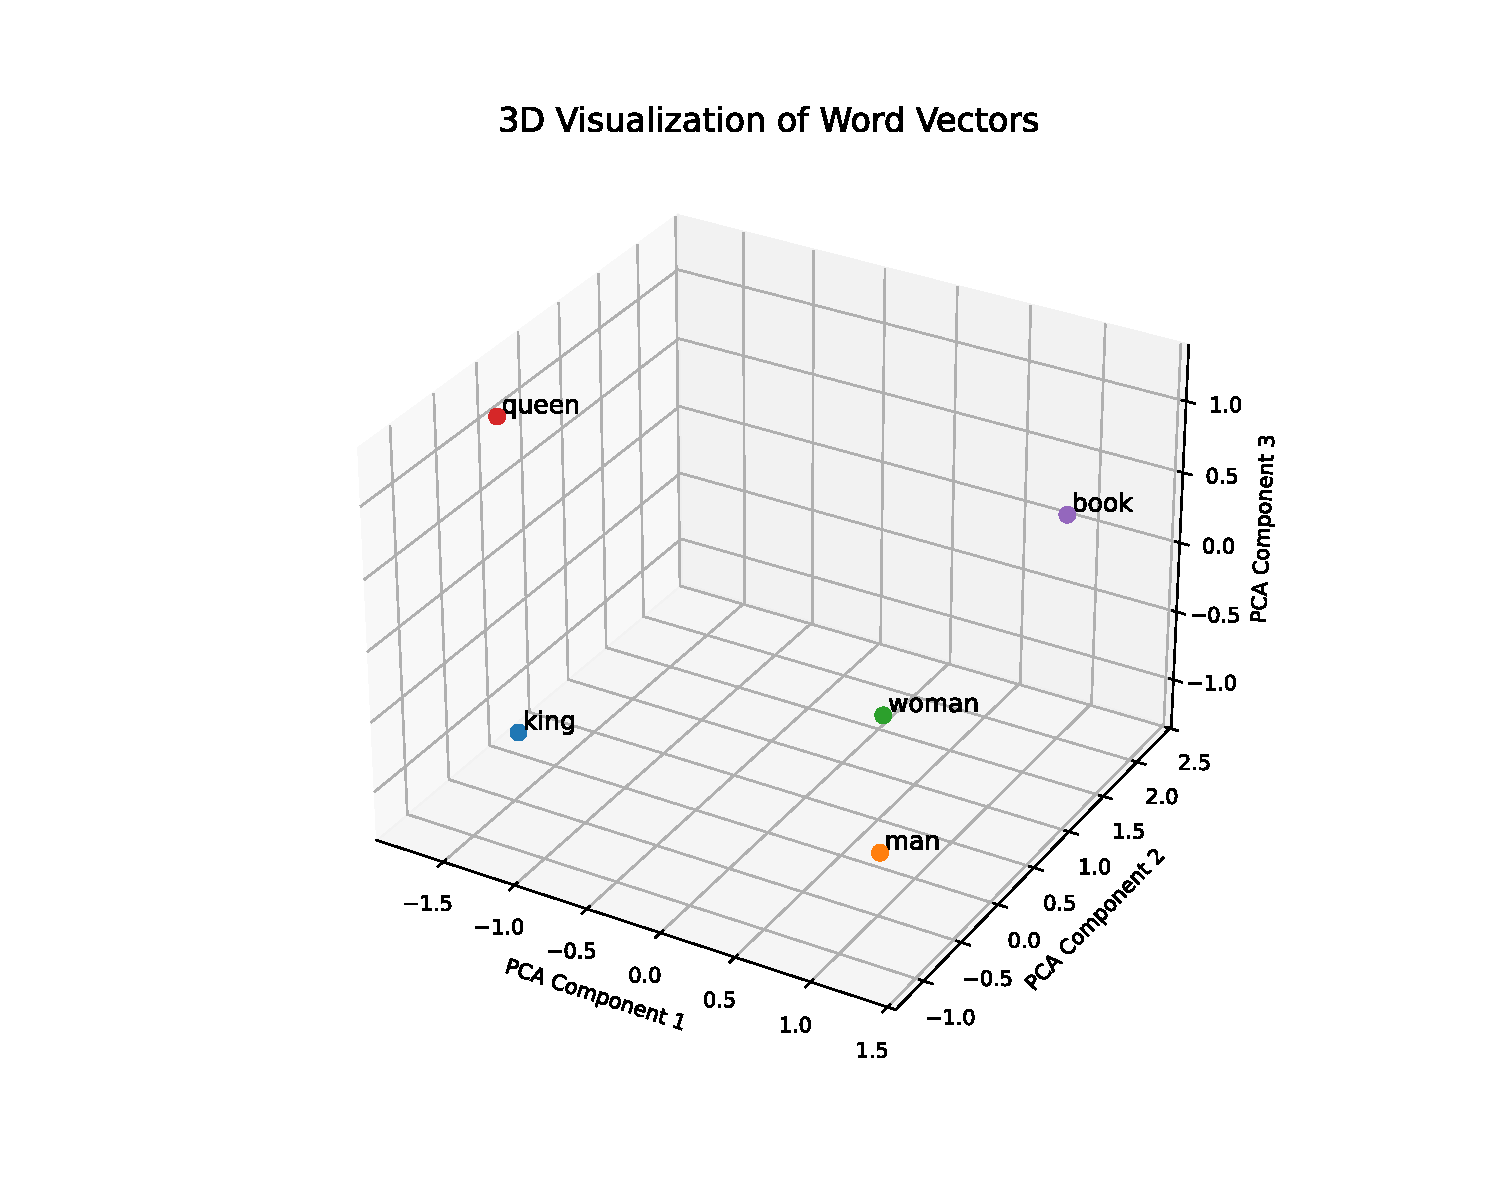
\includegraphics[trim=2cm 2cm 1cm 3cm, clip, width=\linewidth]{figures/word_vector_example.pdf}
    The project used Word2Vec to transform words into high-dimensional vectors, capturing semantic relationships between words. Unlike one-hot encoding, which creates sparse vectors, Word2Vec generates dense vectors where similar words have similar representations in vector space. The model was trained with a custom dataset using Skip-Gram and Continuous Bag of Words (CBOW) techniques to learn word embeddings.
    To measure the similarity between vectors, cosine similarity was employed, which calculates the cosine of the angle between vectors.
    Principal Component Analysis (PCA) was used to reduce the dimensionality of word vectors for a better visualization, helping to observe patterns and clusters of similar words.

    \begin{tikzpicture}
    % Draw a grid
    \draw[step=0.5,gray!30,thin] (-1,-1) grid (4,3);
    
    % Draw coordinate axes
    \draw[->] (-1,0) -- (4,0) node[right] {$x$};
    \draw[->] (0,-1) -- (0,3) node[above] {$y$};
    
    % Draw vectors
    \draw[->,thick,blue] (0,0) -- (3,2) node[midway,below right] {$\vec{u}$};
    \draw[->,thick,red] (0,0) -- (3,0) node[midway,below] {$\vec{v}$};
    
    % Draw angle between vectors
    \draw[->] (1.1,0) arc[start angle=0,end angle=33.69,radius=1cm];
    \node at (1.3,0.3) {$\theta$};
    
    % Draw dotted projections
    \draw[dotted] (3,2) -- (3,0);
    
    % Add labels
    \node at (3.2,1) {\small $\|\vec{u}\|\cos\theta$};
    
    % Enhance the origin
    \fill[black] (0,0) circle (0.05);
\end{tikzpicture}
\end{multicols}

\section{Results}
We tested the performance of our semantic search engine using 10 real-world queries. The results were evaluated using the MRR metric, which assesses the rank of the correct result across multiple queries. The system performed well, with queries such as “NVIDIA Alternative Service” and “AI Competition” ranking first with a perfect score of 1.00. Other queries showed mixed results, with an average MRR score of 0.70. A detailed description of the testing methodology can be found in the appendix.


\section{Discussion}

The result of our semantic search engine indicates the significant advantages of using Word2Vec for information retrieval. The high MMR score of the queries like “NVIDIA Alternative Service” and “AI Competition” shows that it can effectively capture the semantic relationship and contextual relevance even when the exact keywords are missing. However, there are queries with a lower average MMR score which proves that it is not fully optimized yet. The potential of it is highly evident. If it is further optimized, we believe it will become mainstream in the foreseeable future. 

\begin{multicols}{2}
    [
    \section{Conclusion}
    ]
    \blindtext
\end{multicols}

\section{Author Contributions}

\begin{table}[H]
    \centering
    \begin{tabularx}{\textwidth}{p{1.7cm}p{3.5cm}X} % X 表示自適應寬度
        \hline
        \textbf{ID} & \textbf{Name} & \textbf{Contributions} \\ 
        \hline
        112550014 & CHUN-CHE TSAI & Developed and delivered project video presentations, including scriptwriting and video production. \\
        \hline
        113550171 & HAO-WEI WU & Focused on the implementation of Word2Vec and the integration of linear algebra techniques. Additionally, contributed as a TeX writer for the project report.\\
        \hline
        113550014 & YU-KAI SU & Assisted in the implementation and testing phase, especially in evaluating the results, and contributed to the main webpage project implementation. \\
        \hline
        113550806 & CHEUK-CHUNG LI & Mainly assisted in the report writing and delivery of the live presentation. \\
        \hline
        113550139 & CHIN-SHUO CHOU & Developed and delivered project video presentations, including scriptwriting and video production. \\
        \hline
    \end{tabularx}
\end{table}

\newpage
\section{References}

\appendix
\section{Author Contributions}
\dots



\section{Test Cases}

\begin{table}[H]
    \begin{tabular}{ll}
    \hline
    Query     & Target                                    \\
    NVIDIA 研替 & NVIDIA 2025 研發替代役/實習開放職缺資訊                \\
    114甄試     & 114學年度碩士班甄試入學第2階段備取生名單及報到注意事項             \\
    甄試名單      & 114學年度碩士班甄試入學第1階段                         \\
    AI競賽      & AI Junior Award 2025                      \\
    書卷獎       & 【學士班】112學年度第2學期書卷獎得獎名單公告                  \\
    導師名單      & 113.10.15更新【學士班】113學年度第一學期大學部導生名單         \\
    特殊選材      & 114學年度資訊工程學系特殊選才招生公告                      \\
    畢業學分      & 【學士班】113學年度資工系學士班「畢業學分預審」作業公告(請於10/11前繳交) \\
    校友 頒獎     & 資訊人院刊- 資訊系友【交大日資工系友回娘家暨傑出系友頒獎典禮】          \\
    學士畢業      & 【學士班】資訊工程學系畢業離系/離校作業公告                   
    \end{tabular}
\end{table}

\section{Code Implementation}

\small
\begin{lstlisting}
import requests
from bs4 import BeautifulSoup
from tqdm import tqdm
from googletrans import Translator
from nltk.tokenize import word_tokenize
from nltk.corpus import stopwords
import numpy as np
from sentence_transformers import SentenceTransformer
from sklearn.metrics.pairwise import cosine_similarity


# Article class definition
class Article:
    def __init__(self, url: str, title: str) -> None:
        self.article_url = url
        self.original_title = title
        self.translated_title = ""

class ArticleCollection:
    def __init__(self):
        self.articles = []

    def add_article(self, article: Article):
        self.articles.append(article)

    def display_titles(self):
        for article in self.articles:
            print(f"Original Title: {article.original_title}")
            print(f"URL: {article.article_url}")
            print("-" * 15)


class ArticleCollectionFromUrl(ArticleCollection):
    def __init__(self, urls=[]):
        super().__init__()
        self.urls = urls

    def fetch_articles(self):
        for url in tqdm(self.urls):
            response = requests.get(url)
            if response.status_code == 200:
                soup = BeautifulSoup(response.text, "html.parser")
                for item in soup.find_all("li", class_="announcement-item"):
                    link_tag = item.find("h2").find("a")
                    title = link_tag.text.strip()
                    href = link_tag["href"]
                    self.add_article(Article(url=href, title=title))
            else:
                print(f"Unable to access site, status code: {response.status_code}")


# Article translation function
translator = Translator()

def translate_articles(articles):
    for article in tqdm(articles):
        article.translated_title = translator.translate(article.original_title, dest="en").text


# Article search functionality
class ArticleSearch:
    def __init__(self, articles):
        self.articles = articles
        self.model = SentenceTransformer("all-mpnet-base-v2")
        self.article_titles = [article.translated_title for article in articles]
        self.article_vectors = self.model.encode(self.article_titles)

    def search(self, query):
        query_vector = self.model.encode([query])
        similarities = np.array([cosine_similarity(query_vector, vector)[0][0] for vector in self.article_vectors])
        return similarities

    def print_suggestions(self, query, k=5):
        similarities = self.search(query)
        suggestions = np.argsort(-similarities)[:k]
        for idx in suggestions:
            print(f"{similarities[idx]:.4f} : {self.articles[idx].translated_title}")
            print(f"\t\t {self.articles[idx].article_url}")
        print(f"Most similar article: {self.articles[suggestions[0]].translated_title}")


# Translate test query
def translate_test_query(test_cases):
    for test_case in test_cases:
        test_case.query = translator.translate(text=test_case.query, dest="en").text


class TestCase:
    def __init__(self, query, target):
        self.query = query
        self.target = target
    
    def get_score(self, article_search):
        similarities = article_search.search(self.query)
        target_idx = next((i for i, article in enumerate(article_search.articles) if self.target in article.original_title), None)
        if target_idx is None:
            return 0
        most_similar_idx = np.argsort(-similarities)
        return 1 / (np.where(most_similar_idx == target_idx)[0][0] + 1) if target_idx in most_similar_idx else 0


# Main program
PAGES = 1
articles = ArticleCollectionFromUrl([f"https://www.cs.nycu.edu.tw/announcements?page={i}" for i in range(1, PAGES+1)])
articles.fetch_articles()
translate_articles(articles.articles)

# Article search
article_search = ArticleSearch(articles.articles)
article_search.print_suggestions("NVIDIA 研替", k=5)

# Define Test Cases (not all of them are shown)
test_cases = [
    TestCase("AI競賽", "AI Junior Award 2025")
]

# Evaulation
def runtest():
    scores = sum([test_case.get_score(article_search) for test_case in test_cases]) / len(test_cases)
    print(f"score: {scores:.3f}")

runtest()
\end{lstlisting}

\end{document}